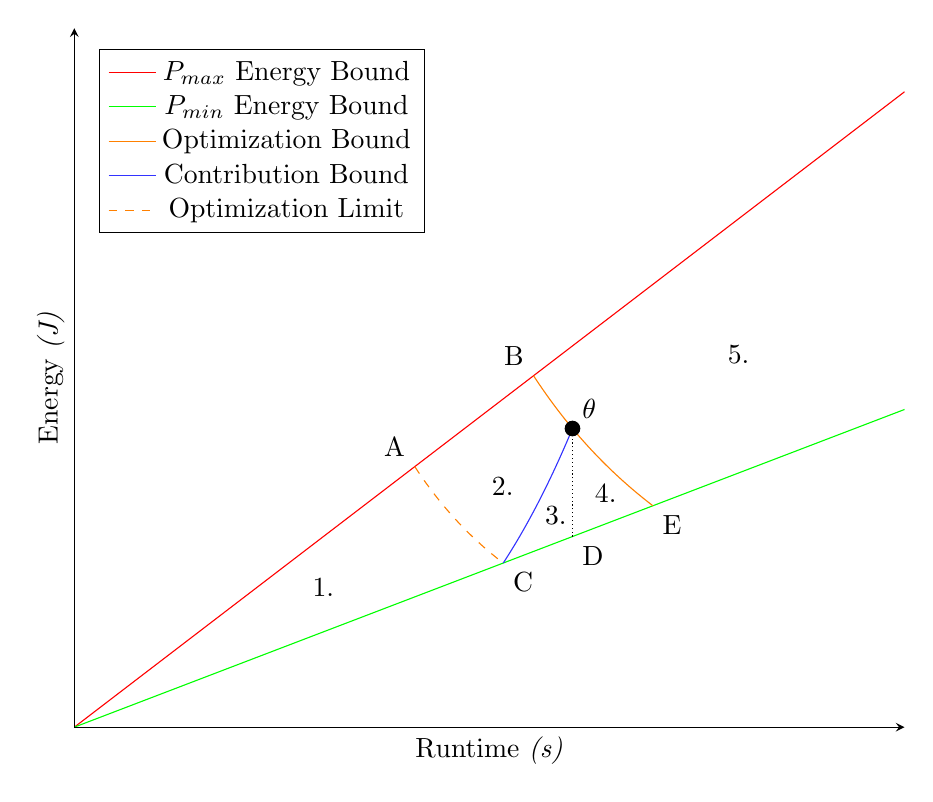
\begin{tikzpicture}
  \begin{axis}[ticks = none, 
    axis on top,
    axis x line=bottom,
    axis y line=left,
  	xlabel={Runtime \emph{(s)}},
    ylabel={Energy \emph{(J)}},    
    xmin=0, xmax=50,
    ymin=0, ymax=3300,
    width=\linewidth,
    legend style={legend pos=north west}
    ]

    %% Model Parameters %%
    \pgfmathsetmacro{\baselinepower}{30} % NOP code
    \pgfmathsetmacro{\rooflinepower}{60}
    \pgfmathsetmacro{\codepower}{47} 
    \pgfmathsetmacro{\codetime}{30}
    % Sadly, pgfplots sucks too much to calculate cube roots
    % These values are calculated with a ruby script in tools
    \pgfmathsetmacro{\blnodex}{25.83028}
    \pgfmathsetmacro{\brnodex}{34.84283}
    \pgfmathsetmacro{\trnodex}{27.65477}
    \pgfmathsetmacro{\tlnodex}{20.50151} % TODO

    %% Intermezzo Values %%
    \pgfmathsetmacro{\brnodey}{\brnodex * \baselinepower}
    \pgfmathsetmacro{\blnodey}{\blnodex * \baselinepower}
    \pgfmathsetmacro{\tlnodey}{\tlnodex * \rooflinepower}
    \pgfmathsetmacro{\trnodey}{\trnodex * \rooflinepower}
    \pgfmathsetmacro{\codeenergy}{\codepower * \codetime}
    \pgfmathsetmacro{\baselineenergy}{\baselinepower * \codetime}


    % arguments: code power, code time, x - todo, apparently not supposed to do pgfmathparse
    \pgfmathdeclarefunction{metricbound}{3}{%
      \pgfmathparse{((#1 * #2^3) / #3^2)}%
    }
    \pgfmathdeclarefunction{definitionbound}{3}{%
      \pgfmathparse{((#1 / #2^3) * #3^4)}%
    }

   % BETA ROOFLINE BOUND 
    \addplot[color=red, domain=\pgfkeysvalueof{/pgfplots/xmin}:\pgfkeysvalueof{/pgfplots/xmax}] {\rooflinepower * x};
    \addlegendentry{$P_{max}$ Energy Bound}

    % ALPHA BASELINE BOUND 
    \addplot[color=green, domain=\pgfkeysvalueof{/pgfplots/xmin}:\pgfkeysvalueof{/pgfplots/xmax}] {\baselinepower * x};
    \addlegendentry{$P_{min}$ Energy Bound} 

    \addplot[color=orange, domain=\trnodex:\brnodex] { metricbound(\codepower, \codetime, x)};
    \addlegendentry{Optimization Bound}

    \addplot[color=blue!80, domain=\blnodex:\codetime] { definitionbound(\codepower, \codetime, x)};
    \addlegendentry{Contribution Bound}

    \addplot[color=orange, dashed, domain=\tlnodex:\blnodex] {metricbound(\baselinepower, \blnodex, x)};
    \addlegendentry{Optimization Limit}

    % Constant Time (Vertical) dotted line
    \draw[densely dotted] ({axis cs:\codetime,\baselineenergy}) -- ({axis cs:\codetime,\codeenergy});

    \node[circle,fill,inner sep=2pt] at (axis cs:\codetime,\codeenergy) {};
    \node[above right] at (axis cs:\codetime,\codeenergy) {$\theta$};
    
    \node [above left] at ({axis cs:\tlnodex, \tlnodey}) {A};
    \node [above left] at ({axis cs:\trnodex, \trnodey}) {B};
    \node [below right] at ({axis cs:\blnodex, \blnodey}) {C};
    \node [below right] at ({axis cs:\codetime,\baselineenergy}) {D};
    \node [below right=0cm] at ({axis cs:\brnodex, \brnodey}) {E};
 

    \pgfmathsetmacro{\onexcoord}{15}
    \node at (axis cs: \onexcoord, 44 * \onexcoord){1.};

    \pgfmathsetmacro{\twoxcoord}{25.8}
    \node at (axis cs: \twoxcoord, 44 * \twoxcoord){2.};

    \pgfmathsetmacro{\threexcoord}{29}
    \node at (axis cs: \threexcoord, 34.5 * \threexcoord){3.};

    \pgfmathsetmacro{\fourxcoord}{32}
    \node at (axis cs: \fourxcoord, 34.5 * \fourxcoord){4.};
    
    \pgfmathsetmacro{\fivexcoord}{40}
    \node at (axis cs: \fivexcoord, 44 * \fivexcoord){5.};
 \end{axis}
\end{tikzpicture}
